\documentclass[12pt, a4paper]{article}
\usepackage{amsmath}
\usepackage{amsfonts}
\usepackage{amsthm}
\usepackage{mathtools}
\newtheorem{theorem}{Theorem}[section]
\newtheorem{definition}{Definition}[section]
\numberwithin{equation}{section}
\usepackage{pgfplots}
\pgfplotsset{width=10cm,compat=1.9}
\graphicspath{ {img/} }
\DeclareGraphicsExtensions{.png, .jpg}

\title{Generalized linear models}
\author{Kristian Wichmann}

\begin{document}
\maketitle

A \textit{generalized linear model} is an extension of the general linear model framework. It introduces a non-linear component to the mean function, and allows the distribution of the response variable to be non-Gaussian.

\section{Components}
A generalized linear model consists of three parts:
\begin{itemize}
\item A stochastic component.
\item A systematic component.
\item A link function.
\end{itemize}

\subsection{Example: Logistic regression}
In simple logistic regression, we try to model the probability of a Bernoulli response variable $y$ as a function of the explanatory variable input $x$, such that:
\begin{equation}
p(x)=\sigma(\beta_1 x+\beta_0)
\end{equation}
Here $\sigma$ is the \textit{logistic function}:
\begin{equation}
\sigma(z)=\frac{1}{1+e^{-z}}
\end{equation}
Figure \ref{fig:logistic_function} graphs the function.

\begin{figure}
\centering
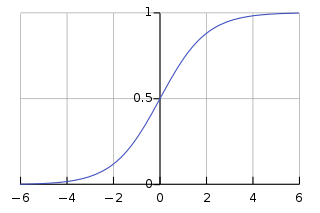
\includegraphics{logistic_function}
\caption{The logistic function $\sigma$.}
\label{fig:logistic_function}
\end{figure}

There's a few important things to note here. First, the parameter $p$ for a Bernoulli distribution is equal to the expectation value. It turns out that it's really the expectation value we wish to model, more generally. Second, the argument of $\sigma$ is linear in the explanatory variable $x$.

\subsection{Stochastic component}
The stochastic component in a generalized linear model is a distribution from the exponential family. The response variable is distributed according to this, with a mean value that is given by the model.

In the logistic regression example above, the stochastic component is the Bernoulli distribution.

\subsection{Systematic component}
The systematic component is the 'linear' part of of the model. I.e. a linear function of the explanatory variables: $X\beta$. Here $\beta$ is a vector of coefficients to be modelled.

In the logistic regression example above, the systematic component is the expression $\beta_1 x+\beta_0$. It is assumed that the constant 1 is an explanatory variable to fit the constant term $\beta_0$ as usual.

\subsection{Link function}
Finally, the link function $g$ is the inverse of the (generally non-linear) function that is applied to the systematic component to get the predicted mean value:
\begin{equation}
\mathbb{E}[y]=g^{-1}(X\beta)
\end{equation}
This of course means, that the function has to be invertible.

In the logistic regression example above, the inverse of the link function is the logistic function:
\begin{equation}
g^{-1}(z)=\sigma(z)
\end{equation}
The link function itself is the inverse, which is known as the \textit{logit} function:
\begin{equation}
g(p)=\ln\left(\frac{p}{1-p}\right)
\end{equation}

\end{document}